\section*{Аннотация}
\textbf{Цель работы:} знакомство с работой и настройкой гониометра Г5,
определение спектральных характеристик амплитудной решётки.\\\indent
\textbf{Оборудование:} гониометр, дифракционная решётка, ртутная лампа.

\section*{Методика измерений}
Внешний вид гониметра представлен на \ref{figure:gonimetr}. Kоллиматор 3, столик 7 и алидада 17 со зрительной трубой 12 крепится на
массивном основании 23.На столике 7 размещаются исследуемые объекты.
Коллиматор закреплён неподвижно, а столик и алидада с трубой могут вращаться
вокруг вертикальной оси.
\begin{figure}[h!]
    \centering
    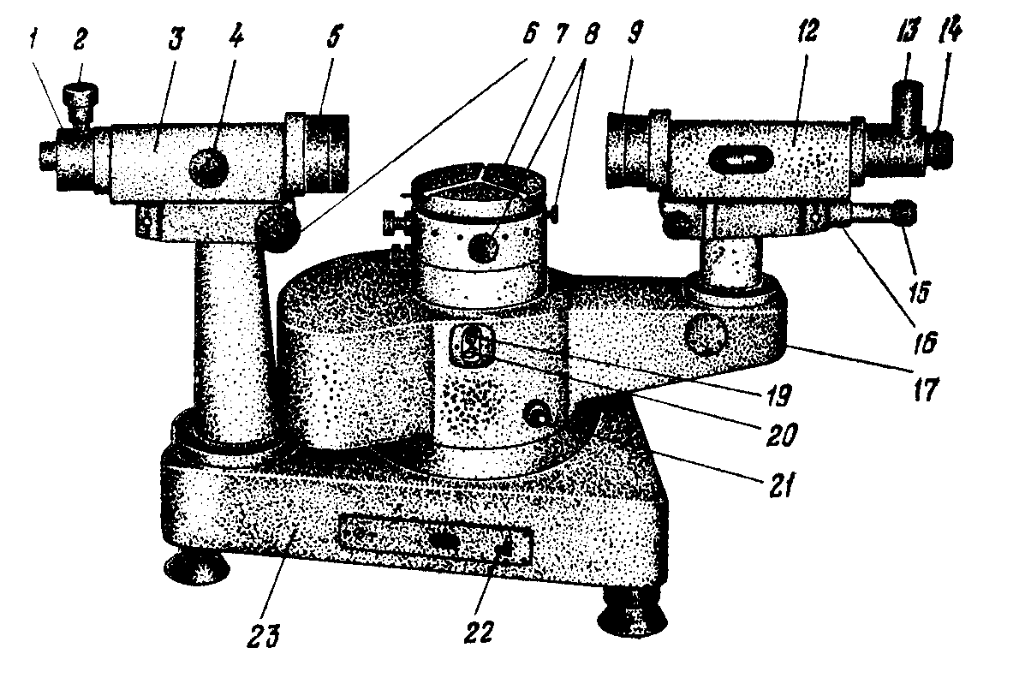
\includegraphics[width=12cm]{images/gonimetr.png}
    \caption{Внешний вид гониметра Г5} \label{figure:gonimetr}
\end{figure}
Ширину коллиматорной щели можно менять от 0 до 2-х мм при помощи
микрометрического винта 2, высоту — от 0 до 20 мм — при помощи диафрагмы с треугольным вырезом, надетой на щель. Винт 4 служит для настройки коллиматора на параллельный пучок.
Зрительная труба 12 состоит из объектива 9 и окуляра 14 с автоколлимационным
устройством 13. Фокусировка трубы производится винтом 11. Наклон коллиматора 
и зрительной трубы к горизонтально оси изменяется винтами 6 и 10 соответственно.

\indent Гониметр требует тщательной юстировки:
Настройка
a) зрительной трубы на бесконечность;
b) поверхности столика и оптической оси трубы — перпендикулярно оси вращения прибора;
c) коллиматора — на параллельный пучок лучей;
d) оптической оси коллиматора - перпендикулярно оси вращения прибора.

\section*{Теоретические сведения}
\begin{wrapfigure}{r}{0.3\linewidth}
    \centering
    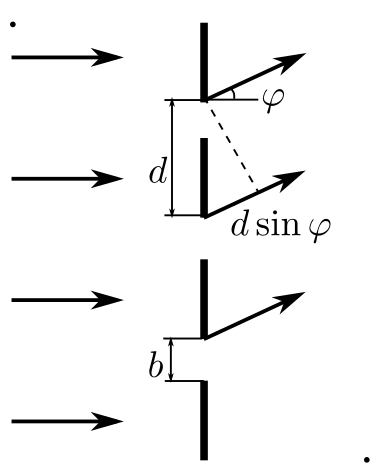
\includegraphics[width=4cm]{images/difrationnaya_reshetka.png}
    \caption{Дифракция световой волны на амплитудной решетке}
\end{wrapfigure}
\indent Амплитудную решётку можно представить в виде непрозрачного экрана, в котором прорезано большое число N параллельных щелей — штрихов. Постоянство 
расстояний между штрихами d и шириной штриха b должно выдерживаться с большой точностью.
\indent Интенсивность дифрагированного света максимальна для углов $\varphi_m$ , при которых волны, приходящие в точку наблюдения от всех щелей, оказываются в
фазе:
\begin{equation}
    d\sin\varphi_m = m\lambda \label{eq:main_difraction}, 
\end{equation}
где $m = 0, \pm 1, \pm 2, \dots$ - порядок спектра.

\indent
Для спектральных приборов важными характеристиками являются
угловая дисперсия, разрешающая способность и дисперсионная область.

\textbf{Разрешающая способность}\\
\begin{equation}
    R = \frac{\lambda}{\delta \lambda} \label{eq:spectr_1}
\end{equation}
\indent Характеризует возможность прибора различать две близкие спектральные линии с длинами волн $\lambda$ и $\lambda + \delta \lambda$.

\textbf{Угловая дисперсия}\\
\begin{equation}
    D = \frac{d\varphi}{d\lambda} = \frac{m}{d\cos\varphi} = \frac{m}{\sqrt{d^2 - m^2{\lambda}^2}} \label{eq:spectr_2}
\end{equation}
\indent По величине угловой дисперсии можно определить угловое расстояния между двумя близкими спектральными линиями.

\textbf{Дисперсионная область}\\
\indent Предельная ширина спектрального интервала $\Delta \lambda$ прибора, для которой дифракционные максимумы соседних порядков не перекрываются. Она определяет диапазон длин волн, при которых прибор может быть использован для
анализа спектра.

\indent Определим угловое расстояние между максимумом линии и её первым нулем — полуширину линии $\delta \varphi$. Пусть на решётку, состоящую из N штрихов, падает параллельный пучок света перпендикулярно её поверхности. Если
N = 2, то две волны погасят друг друга, если между ними возникнет
разность хода $\lambda/2$, если N = 3, то $\lambda/3$. В общем случае N штрихов для полуширины линии $\delta \varphi$ получаем уравнение, решение которого совмест-
но с уравнением \ref{eq:main_difraction} $\delta \varphi \ll 1$ при имеет вид:
\begin{equation}
    d\sin(\varphi_m + \delta \varphi) = m\lambda + \frac{\lambda}{N}
\end{equation}
\begin{equation}
    \delta \varphi = \frac{\lambda}{Nd\cos\varphi_m}
\end{equation}

\indent Тогда с учетом \ref{eq:spectr_2} угловое расстояние между двумя линиями определяется как:
\begin{equation}
    \Delta \varphi \approx D\delta \lambda = \frac{m}{d\cos\varphi_m}\delta \lambda
\end{equation}

\indent Для сравнения между собой различных спектральных приборов Релей предложил приравнять полуширину $\delta \varphi$ и расстояние между лини-
ями $\Delta \varphi$. Критерий Релея удобен для различных оценок. Согласно ему для дифракционных решёток разрешающая способность определяется порядком спектра и числом штрихов:
\begin{equation}
    R = N m
    \label{eq:Reley}
\end{equation}

\section*{Оборудование и инструментальные погрешности}
\noindent\textit{Технические характеристики Г-5:}\\
Поле зрения автоколлиматора: $50'$\\
Предел разрешения автоколлиматора: $30"$\\
Предельная погрешность при измерении угла: $5"$\\
Цена деления шкалы оптического микрометра: $1"$\\
Число штрихов, приходящихся на мм решетки $N$ = 500 штр/мм
\section*{Результаты измерений и обработка данных}

\begin{table}[h!]
    \centering
    \begin{tabular}{|c|c|c|c|c|c|c|c|c|}
        \hline
        Цвет & $\varphi_{1}$ & $\varphi_{-1}$ & Длина волны $\lambda$, нм (эксп) & Длина волны $\lambda$, нм (теор) \\\hline
        K1   & $162^{\circ}10'58"$ & $197^{\circ}50'58"$ & 611.96 & 611.9 \\\hline
        K2   & $162^{\circ}50'58"$ & $198^{\circ}10'58"$ & 623.03 & 623.0 \\\hline
        Ж1   & $163^{\circ}20'58"$ & $196^{\circ}40'58"$ & 573.06 & 577.0 \\\hline
        Ж2   & $163^{\circ}10'58"$ & $196^{\circ}50'58"$ & 578.64 & 579.1 \\\hline
        Г    & $165^{\circ}50'58"$ & $194^{\circ}10'58"$ & 488.94 & 491.6 \\\hline
        C    & $167^{\circ}30'58"$ & $192^{\circ}30'58"$ & 432.33 & 435.8 \\\hline
        Ф    & $168^{\circ}20'58"$ & $191^{\circ}40'58"$ & 403.88 & 404.7 \\\hline
    \end{tabular}
    \caption{Угловые координаты спектральных линий ртути в первом порядке}
\end{table}

$$\sigma_{\lambda} = \sigma_{\varphi} \cos\varphi \cdot d \approx 0.05 \text{ нм}$$

\newpage
\begin{figure}[h!]
    \centering
    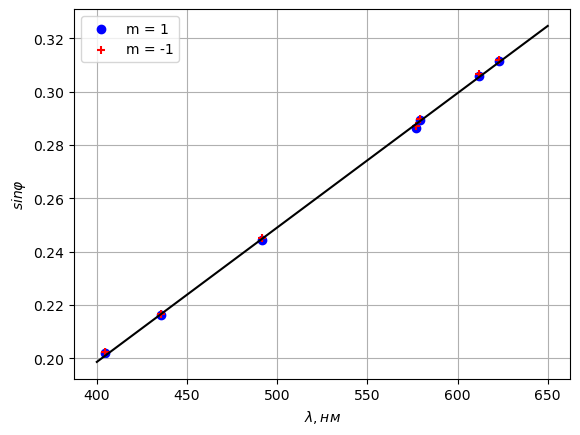
\includegraphics[width=12cm]{images/plot1.png}
    \caption{Зависимость синуса угла спектральных линий в $\pm 1$ порядках от длины волны}
\end{figure}

\indent По графику определим период решетки {\boldmath$d = 1984.8 \pm 0.2$} \textbf{нм}; 
$\sigma_d = \sigma_{\varphi}\cdot \lambda \frac{\cos\varphi}{{\sin^2\varphi}} = 0.2$ нм.

\begin{figure}[h!]
    \centering
    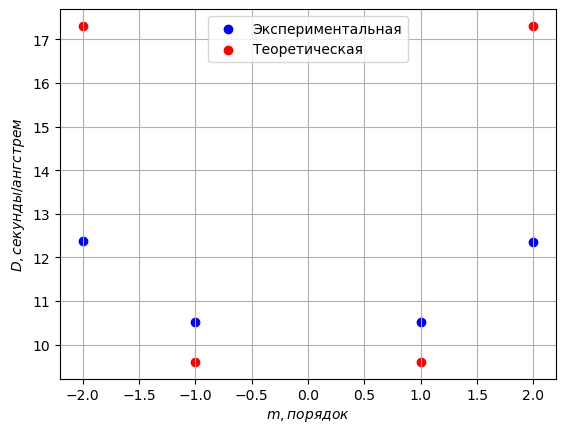
\includegraphics[width=11cm]{images/plot2.png}
    \caption{Зависимость угловой дисперсии желтого спектра от его порядка}
\end{figure}

\begin{table}[h!]
    \centering
    \begin{tabular}{|c|c|c|c|c|}
        \hline
        Порядок m & -2 & -1 & 1 & 2 \\\hline
        Угол  & $215^{\circ}30'58"$ & $196^{\circ}50'58"$ & $163^{\circ}10'58"$ & $144^{\circ}40'58"$ \\\hline
    \end{tabular}
    \caption{Угловые координаты желтого спектра в разных порядках}
\end{table}

\begin{figure}[h!]
    \centering
    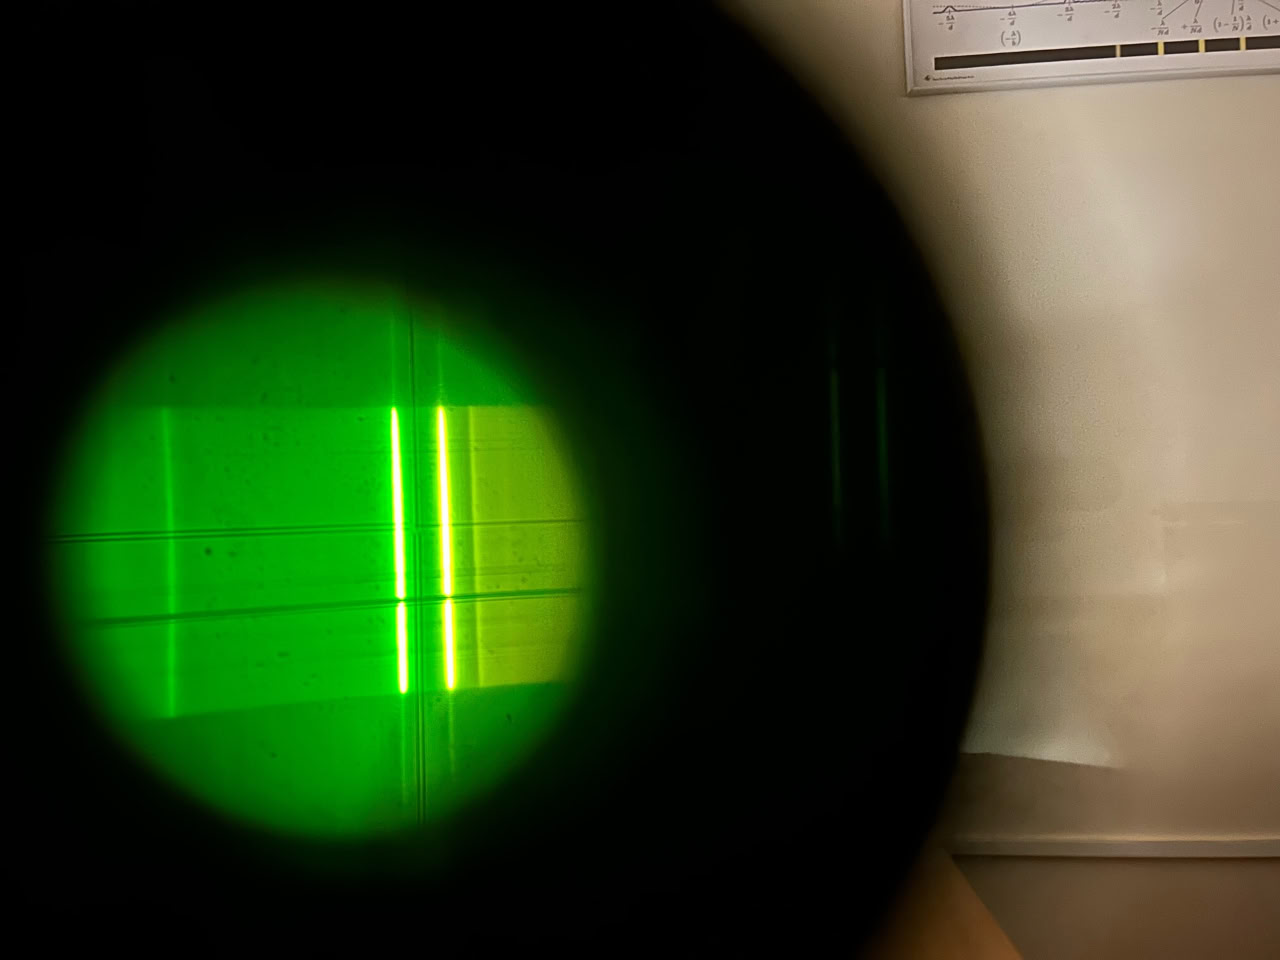
\includegraphics[width=10cm]{images/getR.jpg}
    \caption{Определение разрешающей способности для желтого дублета}
\end{figure}

Для качественного определения аппаратной разрешающей способности $R$ оценим на глаз, во сколько раз расстояние между центрами желтых линий больше полуширины одной линии: $R \approx 12$.

\section*{Обсуждение результатов и выводы}














